\documentclass{article}

\usepackage{tikz}
\usepackage{pgfplots}
\pgfplotsset{compat=newest}
\usepgfplotslibrary{patchplots}

\pagestyle{empty}


%Common symbols
%Common math symbols

%Real Numbers
	\newcommand{\Real}{\mathbb{R}}
% Kinematic Configurations
	\newcommand{\Conf}{\mathrm{C}}
% Atlas
	\newcommand{\Atlas}{\mathcal{A}}

%Lagrangiana
	\newcommand{\Lagrangian}{\mathcal{L}}

%Solutions Space
	\newcommand{\Sol}{\mathrm{Sol}}
\begin{document}


Figura 1: La rappresentazione 2D dello spazio delle configurazioni Cinematiche\\
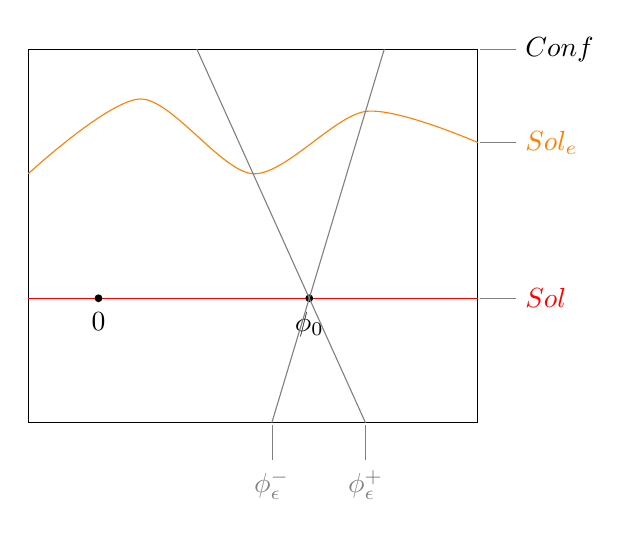
\begin{tikzpicture}

\begin{axis}[axis lines=none,clip=false]

	% Il riquadro di \Conf
	\addplot[color=black] coordinates {
		(8,6) (0,6) (0,0)(8,0)(8,6)
		}node [pos=1,pin={0:$Conf$},inner sep=0pt] {};

	% la retta di \Sol
	\addplot[color=red] coordinates {
		(0,2)
		(8,2)
	}node [pos=1,pin={0:$Sol$},inner sep=0pt] {};
	
	% La curva di \Sol_\epsilon
	\addplot[color=orange,smooth] coordinates {
	(0,4) (2,5.2)(4,4)(6,5)(8,4.5)
	}node [pos=1,pin={0:$Sol_e$},inner sep=0pt] {};

	% Zero section
	\node[label={270:{$0$}},circle,fill,inner sep=1pt] at (axis cs:1.25,2) {};
	% Fixed Solution
	\node[label={270:{$\phi_0$}},circle,fill,inner sep=1pt] at (axis cs:5,2) {};

	%Perturbation
	\addplot[color=gray] coordinates {
		(3,6)
		(6,0)
	}node [pos=1,pin={270:$\phi_\epsilon^+$},inner sep=0pt] {};
	\addplot[color=gray] coordinates {
		(6.33333,6)
		(4.33333,0)
	}node [pos=1,pin={270:$\phi_\epsilon^-$},inner sep=0pt] {};

\end{axis}
\end{tikzpicture}






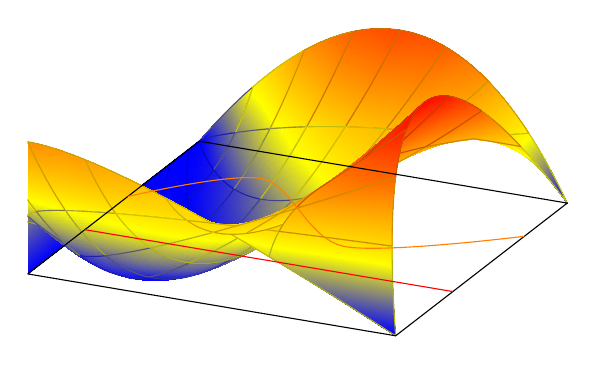
\begin{tikzpicture}
\begin{axis}[axis lines=none]

\addplot3[patch,patch type=biquadratic,
	shader=faceted interp,patch refines=3]
coordinates {
	(0,0,5) (8,0,5) (8,6,5) (0,6,5)
	(0,0,6) (8,1,6.6) (5,5,6.3) (0,5,5)
	(3,1,5)
};


	\addplot[color=black] coordinates {
		(0,0) (8,0) (8,6) (0,6) (0,0)
		};

	\addplot[color=red] coordinates {
		(0,2)
		(8,2)
	};
	
	\addplot[color=orange,smooth] coordinates {
	(0,3.5) (2,5)(5,3)(8,4.5)
	};



\end{axis}
\end{tikzpicture}
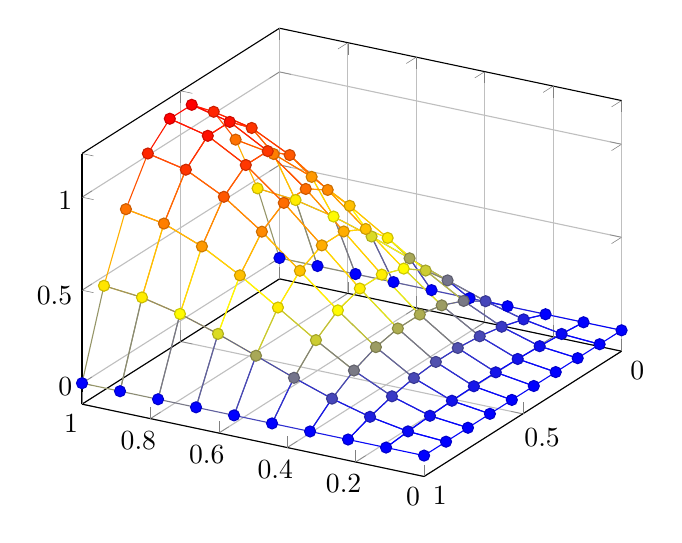
\begin{tikzpicture}
	\begin{axis}[grid=major,view={210}{30}]
	\addplot3+[mesh,scatter,samples=10,domain=0:1] 
		{5*x*sin(2*deg(x)) * y*(1-y)};
	\end{axis}
\end{tikzpicture}

\end{document}

